
% Default to the notebook output style

    


% Inherit from the specified cell style.




    
\documentclass[11pt]{article}

    
    
    \usepackage[T1]{fontenc}
    % Nicer default font (+ math font) than Computer Modern for most use cases
    \usepackage{mathpazo}

    % Basic figure setup, for now with no caption control since it's done
    % automatically by Pandoc (which extracts ![](path) syntax from Markdown).
    \usepackage{graphicx}
    % We will generate all images so they have a width \maxwidth. This means
    % that they will get their normal width if they fit onto the page, but
    % are scaled down if they would overflow the margins.
    \makeatletter
    \def\maxwidth{\ifdim\Gin@nat@width>\linewidth\linewidth
    \else\Gin@nat@width\fi}
    \makeatother
    \let\Oldincludegraphics\includegraphics
    % Set max figure width to be 80% of text width, for now hardcoded.
    \renewcommand{\includegraphics}[1]{\Oldincludegraphics[width=.8\maxwidth]{#1}}
    % Ensure that by default, figures have no caption (until we provide a
    % proper Figure object with a Caption API and a way to capture that
    % in the conversion process - todo).
    \usepackage{caption}
    \DeclareCaptionLabelFormat{nolabel}{}
    \captionsetup{labelformat=nolabel}

    \usepackage{adjustbox} % Used to constrain images to a maximum size 
    \usepackage{xcolor} % Allow colors to be defined
    \usepackage{enumerate} % Needed for markdown enumerations to work
    \usepackage{geometry} % Used to adjust the document margins
    \usepackage{amsmath} % Equations
    \usepackage{amssymb} % Equations
    \usepackage{textcomp} % defines textquotesingle
    % Hack from http://tex.stackexchange.com/a/47451/13684:
    \AtBeginDocument{%
        \def\PYZsq{\textquotesingle}% Upright quotes in Pygmentized code
    }
    \usepackage{upquote} % Upright quotes for verbatim code
    \usepackage{eurosym} % defines \euro
    \usepackage[mathletters]{ucs} % Extended unicode (utf-8) support
    \usepackage[utf8x]{inputenc} % Allow utf-8 characters in the tex document
    \usepackage{fancyvrb} % verbatim replacement that allows latex
    \usepackage{grffile} % extends the file name processing of package graphics 
                         % to support a larger range 
    % The hyperref package gives us a pdf with properly built
    % internal navigation ('pdf bookmarks' for the table of contents,
    % internal cross-reference links, web links for URLs, etc.)
    \usepackage{hyperref}
    \usepackage{longtable} % longtable support required by pandoc >1.10
    \usepackage{booktabs}  % table support for pandoc > 1.12.2
    \usepackage[inline]{enumitem} % IRkernel/repr support (it uses the enumerate* environment)
    \usepackage[normalem]{ulem} % ulem is needed to support strikethroughs (\sout)
                                % normalem makes italics be italics, not underlines
    

    
    
    % Colors for the hyperref package
    \definecolor{urlcolor}{rgb}{0,.145,.698}
    \definecolor{linkcolor}{rgb}{.71,0.21,0.01}
    \definecolor{citecolor}{rgb}{.12,.54,.11}

    % ANSI colors
    \definecolor{ansi-black}{HTML}{3E424D}
    \definecolor{ansi-black-intense}{HTML}{282C36}
    \definecolor{ansi-red}{HTML}{E75C58}
    \definecolor{ansi-red-intense}{HTML}{B22B31}
    \definecolor{ansi-green}{HTML}{00A250}
    \definecolor{ansi-green-intense}{HTML}{007427}
    \definecolor{ansi-yellow}{HTML}{DDB62B}
    \definecolor{ansi-yellow-intense}{HTML}{B27D12}
    \definecolor{ansi-blue}{HTML}{208FFB}
    \definecolor{ansi-blue-intense}{HTML}{0065CA}
    \definecolor{ansi-magenta}{HTML}{D160C4}
    \definecolor{ansi-magenta-intense}{HTML}{A03196}
    \definecolor{ansi-cyan}{HTML}{60C6C8}
    \definecolor{ansi-cyan-intense}{HTML}{258F8F}
    \definecolor{ansi-white}{HTML}{C5C1B4}
    \definecolor{ansi-white-intense}{HTML}{A1A6B2}

    % commands and environments needed by pandoc snippets
    % extracted from the output of `pandoc -s`
    \providecommand{\tightlist}{%
      \setlength{\itemsep}{0pt}\setlength{\parskip}{0pt}}
    \DefineVerbatimEnvironment{Highlighting}{Verbatim}{commandchars=\\\{\}}
    % Add ',fontsize=\small' for more characters per line
    \newenvironment{Shaded}{}{}
    \newcommand{\KeywordTok}[1]{\textcolor[rgb]{0.00,0.44,0.13}{\textbf{{#1}}}}
    \newcommand{\DataTypeTok}[1]{\textcolor[rgb]{0.56,0.13,0.00}{{#1}}}
    \newcommand{\DecValTok}[1]{\textcolor[rgb]{0.25,0.63,0.44}{{#1}}}
    \newcommand{\BaseNTok}[1]{\textcolor[rgb]{0.25,0.63,0.44}{{#1}}}
    \newcommand{\FloatTok}[1]{\textcolor[rgb]{0.25,0.63,0.44}{{#1}}}
    \newcommand{\CharTok}[1]{\textcolor[rgb]{0.25,0.44,0.63}{{#1}}}
    \newcommand{\StringTok}[1]{\textcolor[rgb]{0.25,0.44,0.63}{{#1}}}
    \newcommand{\CommentTok}[1]{\textcolor[rgb]{0.38,0.63,0.69}{\textit{{#1}}}}
    \newcommand{\OtherTok}[1]{\textcolor[rgb]{0.00,0.44,0.13}{{#1}}}
    \newcommand{\AlertTok}[1]{\textcolor[rgb]{1.00,0.00,0.00}{\textbf{{#1}}}}
    \newcommand{\FunctionTok}[1]{\textcolor[rgb]{0.02,0.16,0.49}{{#1}}}
    \newcommand{\RegionMarkerTok}[1]{{#1}}
    \newcommand{\ErrorTok}[1]{\textcolor[rgb]{1.00,0.00,0.00}{\textbf{{#1}}}}
    \newcommand{\NormalTok}[1]{{#1}}
    
    % Additional commands for more recent versions of Pandoc
    \newcommand{\ConstantTok}[1]{\textcolor[rgb]{0.53,0.00,0.00}{{#1}}}
    \newcommand{\SpecialCharTok}[1]{\textcolor[rgb]{0.25,0.44,0.63}{{#1}}}
    \newcommand{\VerbatimStringTok}[1]{\textcolor[rgb]{0.25,0.44,0.63}{{#1}}}
    \newcommand{\SpecialStringTok}[1]{\textcolor[rgb]{0.73,0.40,0.53}{{#1}}}
    \newcommand{\ImportTok}[1]{{#1}}
    \newcommand{\DocumentationTok}[1]{\textcolor[rgb]{0.73,0.13,0.13}{\textit{{#1}}}}
    \newcommand{\AnnotationTok}[1]{\textcolor[rgb]{0.38,0.63,0.69}{\textbf{\textit{{#1}}}}}
    \newcommand{\CommentVarTok}[1]{\textcolor[rgb]{0.38,0.63,0.69}{\textbf{\textit{{#1}}}}}
    \newcommand{\VariableTok}[1]{\textcolor[rgb]{0.10,0.09,0.49}{{#1}}}
    \newcommand{\ControlFlowTok}[1]{\textcolor[rgb]{0.00,0.44,0.13}{\textbf{{#1}}}}
    \newcommand{\OperatorTok}[1]{\textcolor[rgb]{0.40,0.40,0.40}{{#1}}}
    \newcommand{\BuiltInTok}[1]{{#1}}
    \newcommand{\ExtensionTok}[1]{{#1}}
    \newcommand{\PreprocessorTok}[1]{\textcolor[rgb]{0.74,0.48,0.00}{{#1}}}
    \newcommand{\AttributeTok}[1]{\textcolor[rgb]{0.49,0.56,0.16}{{#1}}}
    \newcommand{\InformationTok}[1]{\textcolor[rgb]{0.38,0.63,0.69}{\textbf{\textit{{#1}}}}}
    \newcommand{\WarningTok}[1]{\textcolor[rgb]{0.38,0.63,0.69}{\textbf{\textit{{#1}}}}}
    
    
    % Define a nice break command that doesn't care if a line doesn't already
    % exist.
    \def\br{\hspace*{\fill} \\* }
    % Math Jax compatability definitions
    \def\gt{>}
    \def\lt{<}
    % Document parameters
    \title{Exercise 1  Virtual World Contruction}
    
    
    

    % Pygments definitions
    
\makeatletter
\def\PY@reset{\let\PY@it=\relax \let\PY@bf=\relax%
    \let\PY@ul=\relax \let\PY@tc=\relax%
    \let\PY@bc=\relax \let\PY@ff=\relax}
\def\PY@tok#1{\csname PY@tok@#1\endcsname}
\def\PY@toks#1+{\ifx\relax#1\empty\else%
    \PY@tok{#1}\expandafter\PY@toks\fi}
\def\PY@do#1{\PY@bc{\PY@tc{\PY@ul{%
    \PY@it{\PY@bf{\PY@ff{#1}}}}}}}
\def\PY#1#2{\PY@reset\PY@toks#1+\relax+\PY@do{#2}}

\expandafter\def\csname PY@tok@gd\endcsname{\def\PY@tc##1{\textcolor[rgb]{0.63,0.00,0.00}{##1}}}
\expandafter\def\csname PY@tok@gu\endcsname{\let\PY@bf=\textbf\def\PY@tc##1{\textcolor[rgb]{0.50,0.00,0.50}{##1}}}
\expandafter\def\csname PY@tok@gt\endcsname{\def\PY@tc##1{\textcolor[rgb]{0.00,0.27,0.87}{##1}}}
\expandafter\def\csname PY@tok@gs\endcsname{\let\PY@bf=\textbf}
\expandafter\def\csname PY@tok@gr\endcsname{\def\PY@tc##1{\textcolor[rgb]{1.00,0.00,0.00}{##1}}}
\expandafter\def\csname PY@tok@cm\endcsname{\let\PY@it=\textit\def\PY@tc##1{\textcolor[rgb]{0.25,0.50,0.50}{##1}}}
\expandafter\def\csname PY@tok@vg\endcsname{\def\PY@tc##1{\textcolor[rgb]{0.10,0.09,0.49}{##1}}}
\expandafter\def\csname PY@tok@vi\endcsname{\def\PY@tc##1{\textcolor[rgb]{0.10,0.09,0.49}{##1}}}
\expandafter\def\csname PY@tok@vm\endcsname{\def\PY@tc##1{\textcolor[rgb]{0.10,0.09,0.49}{##1}}}
\expandafter\def\csname PY@tok@mh\endcsname{\def\PY@tc##1{\textcolor[rgb]{0.40,0.40,0.40}{##1}}}
\expandafter\def\csname PY@tok@cs\endcsname{\let\PY@it=\textit\def\PY@tc##1{\textcolor[rgb]{0.25,0.50,0.50}{##1}}}
\expandafter\def\csname PY@tok@ge\endcsname{\let\PY@it=\textit}
\expandafter\def\csname PY@tok@vc\endcsname{\def\PY@tc##1{\textcolor[rgb]{0.10,0.09,0.49}{##1}}}
\expandafter\def\csname PY@tok@il\endcsname{\def\PY@tc##1{\textcolor[rgb]{0.40,0.40,0.40}{##1}}}
\expandafter\def\csname PY@tok@go\endcsname{\def\PY@tc##1{\textcolor[rgb]{0.53,0.53,0.53}{##1}}}
\expandafter\def\csname PY@tok@cp\endcsname{\def\PY@tc##1{\textcolor[rgb]{0.74,0.48,0.00}{##1}}}
\expandafter\def\csname PY@tok@gi\endcsname{\def\PY@tc##1{\textcolor[rgb]{0.00,0.63,0.00}{##1}}}
\expandafter\def\csname PY@tok@gh\endcsname{\let\PY@bf=\textbf\def\PY@tc##1{\textcolor[rgb]{0.00,0.00,0.50}{##1}}}
\expandafter\def\csname PY@tok@ni\endcsname{\let\PY@bf=\textbf\def\PY@tc##1{\textcolor[rgb]{0.60,0.60,0.60}{##1}}}
\expandafter\def\csname PY@tok@nl\endcsname{\def\PY@tc##1{\textcolor[rgb]{0.63,0.63,0.00}{##1}}}
\expandafter\def\csname PY@tok@nn\endcsname{\let\PY@bf=\textbf\def\PY@tc##1{\textcolor[rgb]{0.00,0.00,1.00}{##1}}}
\expandafter\def\csname PY@tok@no\endcsname{\def\PY@tc##1{\textcolor[rgb]{0.53,0.00,0.00}{##1}}}
\expandafter\def\csname PY@tok@na\endcsname{\def\PY@tc##1{\textcolor[rgb]{0.49,0.56,0.16}{##1}}}
\expandafter\def\csname PY@tok@nb\endcsname{\def\PY@tc##1{\textcolor[rgb]{0.00,0.50,0.00}{##1}}}
\expandafter\def\csname PY@tok@nc\endcsname{\let\PY@bf=\textbf\def\PY@tc##1{\textcolor[rgb]{0.00,0.00,1.00}{##1}}}
\expandafter\def\csname PY@tok@nd\endcsname{\def\PY@tc##1{\textcolor[rgb]{0.67,0.13,1.00}{##1}}}
\expandafter\def\csname PY@tok@ne\endcsname{\let\PY@bf=\textbf\def\PY@tc##1{\textcolor[rgb]{0.82,0.25,0.23}{##1}}}
\expandafter\def\csname PY@tok@nf\endcsname{\def\PY@tc##1{\textcolor[rgb]{0.00,0.00,1.00}{##1}}}
\expandafter\def\csname PY@tok@si\endcsname{\let\PY@bf=\textbf\def\PY@tc##1{\textcolor[rgb]{0.73,0.40,0.53}{##1}}}
\expandafter\def\csname PY@tok@s2\endcsname{\def\PY@tc##1{\textcolor[rgb]{0.73,0.13,0.13}{##1}}}
\expandafter\def\csname PY@tok@nt\endcsname{\let\PY@bf=\textbf\def\PY@tc##1{\textcolor[rgb]{0.00,0.50,0.00}{##1}}}
\expandafter\def\csname PY@tok@nv\endcsname{\def\PY@tc##1{\textcolor[rgb]{0.10,0.09,0.49}{##1}}}
\expandafter\def\csname PY@tok@s1\endcsname{\def\PY@tc##1{\textcolor[rgb]{0.73,0.13,0.13}{##1}}}
\expandafter\def\csname PY@tok@dl\endcsname{\def\PY@tc##1{\textcolor[rgb]{0.73,0.13,0.13}{##1}}}
\expandafter\def\csname PY@tok@ch\endcsname{\let\PY@it=\textit\def\PY@tc##1{\textcolor[rgb]{0.25,0.50,0.50}{##1}}}
\expandafter\def\csname PY@tok@m\endcsname{\def\PY@tc##1{\textcolor[rgb]{0.40,0.40,0.40}{##1}}}
\expandafter\def\csname PY@tok@gp\endcsname{\let\PY@bf=\textbf\def\PY@tc##1{\textcolor[rgb]{0.00,0.00,0.50}{##1}}}
\expandafter\def\csname PY@tok@sh\endcsname{\def\PY@tc##1{\textcolor[rgb]{0.73,0.13,0.13}{##1}}}
\expandafter\def\csname PY@tok@ow\endcsname{\let\PY@bf=\textbf\def\PY@tc##1{\textcolor[rgb]{0.67,0.13,1.00}{##1}}}
\expandafter\def\csname PY@tok@sx\endcsname{\def\PY@tc##1{\textcolor[rgb]{0.00,0.50,0.00}{##1}}}
\expandafter\def\csname PY@tok@bp\endcsname{\def\PY@tc##1{\textcolor[rgb]{0.00,0.50,0.00}{##1}}}
\expandafter\def\csname PY@tok@c1\endcsname{\let\PY@it=\textit\def\PY@tc##1{\textcolor[rgb]{0.25,0.50,0.50}{##1}}}
\expandafter\def\csname PY@tok@fm\endcsname{\def\PY@tc##1{\textcolor[rgb]{0.00,0.00,1.00}{##1}}}
\expandafter\def\csname PY@tok@o\endcsname{\def\PY@tc##1{\textcolor[rgb]{0.40,0.40,0.40}{##1}}}
\expandafter\def\csname PY@tok@kc\endcsname{\let\PY@bf=\textbf\def\PY@tc##1{\textcolor[rgb]{0.00,0.50,0.00}{##1}}}
\expandafter\def\csname PY@tok@c\endcsname{\let\PY@it=\textit\def\PY@tc##1{\textcolor[rgb]{0.25,0.50,0.50}{##1}}}
\expandafter\def\csname PY@tok@mf\endcsname{\def\PY@tc##1{\textcolor[rgb]{0.40,0.40,0.40}{##1}}}
\expandafter\def\csname PY@tok@err\endcsname{\def\PY@bc##1{\setlength{\fboxsep}{0pt}\fcolorbox[rgb]{1.00,0.00,0.00}{1,1,1}{\strut ##1}}}
\expandafter\def\csname PY@tok@mb\endcsname{\def\PY@tc##1{\textcolor[rgb]{0.40,0.40,0.40}{##1}}}
\expandafter\def\csname PY@tok@ss\endcsname{\def\PY@tc##1{\textcolor[rgb]{0.10,0.09,0.49}{##1}}}
\expandafter\def\csname PY@tok@sr\endcsname{\def\PY@tc##1{\textcolor[rgb]{0.73,0.40,0.53}{##1}}}
\expandafter\def\csname PY@tok@mo\endcsname{\def\PY@tc##1{\textcolor[rgb]{0.40,0.40,0.40}{##1}}}
\expandafter\def\csname PY@tok@kd\endcsname{\let\PY@bf=\textbf\def\PY@tc##1{\textcolor[rgb]{0.00,0.50,0.00}{##1}}}
\expandafter\def\csname PY@tok@mi\endcsname{\def\PY@tc##1{\textcolor[rgb]{0.40,0.40,0.40}{##1}}}
\expandafter\def\csname PY@tok@kn\endcsname{\let\PY@bf=\textbf\def\PY@tc##1{\textcolor[rgb]{0.00,0.50,0.00}{##1}}}
\expandafter\def\csname PY@tok@cpf\endcsname{\let\PY@it=\textit\def\PY@tc##1{\textcolor[rgb]{0.25,0.50,0.50}{##1}}}
\expandafter\def\csname PY@tok@kr\endcsname{\let\PY@bf=\textbf\def\PY@tc##1{\textcolor[rgb]{0.00,0.50,0.00}{##1}}}
\expandafter\def\csname PY@tok@s\endcsname{\def\PY@tc##1{\textcolor[rgb]{0.73,0.13,0.13}{##1}}}
\expandafter\def\csname PY@tok@kp\endcsname{\def\PY@tc##1{\textcolor[rgb]{0.00,0.50,0.00}{##1}}}
\expandafter\def\csname PY@tok@w\endcsname{\def\PY@tc##1{\textcolor[rgb]{0.73,0.73,0.73}{##1}}}
\expandafter\def\csname PY@tok@kt\endcsname{\def\PY@tc##1{\textcolor[rgb]{0.69,0.00,0.25}{##1}}}
\expandafter\def\csname PY@tok@sc\endcsname{\def\PY@tc##1{\textcolor[rgb]{0.73,0.13,0.13}{##1}}}
\expandafter\def\csname PY@tok@sb\endcsname{\def\PY@tc##1{\textcolor[rgb]{0.73,0.13,0.13}{##1}}}
\expandafter\def\csname PY@tok@sa\endcsname{\def\PY@tc##1{\textcolor[rgb]{0.73,0.13,0.13}{##1}}}
\expandafter\def\csname PY@tok@k\endcsname{\let\PY@bf=\textbf\def\PY@tc##1{\textcolor[rgb]{0.00,0.50,0.00}{##1}}}
\expandafter\def\csname PY@tok@se\endcsname{\let\PY@bf=\textbf\def\PY@tc##1{\textcolor[rgb]{0.73,0.40,0.13}{##1}}}
\expandafter\def\csname PY@tok@sd\endcsname{\let\PY@it=\textit\def\PY@tc##1{\textcolor[rgb]{0.73,0.13,0.13}{##1}}}

\def\PYZbs{\char`\\}
\def\PYZus{\char`\_}
\def\PYZob{\char`\{}
\def\PYZcb{\char`\}}
\def\PYZca{\char`\^}
\def\PYZam{\char`\&}
\def\PYZlt{\char`\<}
\def\PYZgt{\char`\>}
\def\PYZsh{\char`\#}
\def\PYZpc{\char`\%}
\def\PYZdl{\char`\$}
\def\PYZhy{\char`\-}
\def\PYZsq{\char`\'}
\def\PYZdq{\char`\"}
\def\PYZti{\char`\~}
% for compatibility with earlier versions
\def\PYZat{@}
\def\PYZlb{[}
\def\PYZrb{]}
\makeatother


    % Exact colors from NB
    \definecolor{incolor}{rgb}{0.0, 0.0, 0.5}
    \definecolor{outcolor}{rgb}{0.545, 0.0, 0.0}



    
    % Prevent overflowing lines due to hard-to-break entities
    \sloppy 
    % Setup hyperref package
    \hypersetup{
      breaklinks=true,  % so long urls are correctly broken across lines
      colorlinks=true,
      urlcolor=urlcolor,
      linkcolor=linkcolor,
      citecolor=citecolor,
      }
    % Slightly bigger margins than the latex defaults
    
    \geometry{verbose,tmargin=1in,bmargin=1in,lmargin=1in,rmargin=1in}
    
    

    \begin{document}
    
    
    \maketitle
    
    

    
    *** Xiangyi Cheng (xxc283)***

    \hypertarget{concept-and-background}{%
\section{Concept and Background}\label{concept-and-background}}

    The aim of this exercise is to build a 3D virtual world with a set of
points and set two cameras in different locations. The cameras should be
defined by position, target, up, focal length, film width, film height.
The numbers of horizontal and vertical pixel of the images taken by the
cameras are specified as width and height.

The camera is a mapping between the 3D world and a 2D image. Projection
is how the camera convert the 3D object into 2D image. There are several
camera models, such as finite cameras, the projective camera, cameras at
infinity, etc.. The most specialized and simplest model among them is
called the basic pinhole camera. Before deeping into the projection
concept, we have to understand another two terms called the world
coordinate frame and the camera coordinate frame. The world coordinate
frame is the frame we define the location of the points and the cameras
while the camera coordinate frame whose center is the camera position
which we will use to compute the projection plane corner points as shown
below. The camera coordinate frame could be calculated based on the
camera parameters.

\begin{figure}
\centering
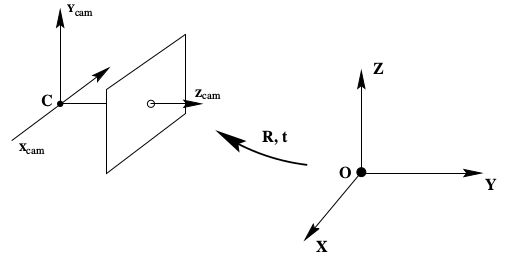
\includegraphics{trans.png}
\caption{world coordinate frame and camera coordinate frame}
\end{figure}

After obtaining the coordiantes, the image below illustrates the
projection in terms of a ponhole camera which belongs to finite camera
category. C is the camera center and the distance between C and P is the
focal length. X represents the object in 3D world while x is projected
location in the image. Based on the known focal width, focal lengt and
the distance from the target position to the real position of the
objects, we are able to calculate the projective plane by applying the
similar triangle rule.

\begin{figure}
\centering
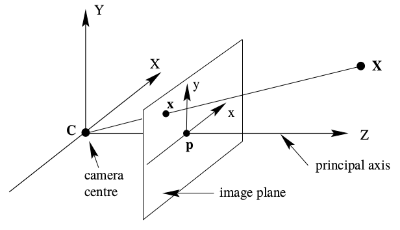
\includegraphics{pro.png}
\caption{projection}
\end{figure}

Below is an example shows how to build a set of points in a 3D virtual
world and the projection by two cameras set in different position and
angles.

    \hypertarget{implement-and-exploration}{%
\section{Implement and Exploration}\label{implement-and-exploration}}

    The code is developed in python. Import several useful libraries which
will be used later at the beginning.

    \begin{Verbatim}[commandchars=\\\{\}]
{\color{incolor}In [{\color{incolor}1}]:} \PY{k+kn}{import} \PY{n+nn}{numpy} \PY{k+kn}{as} \PY{n+nn}{np}
        \PY{k+kn}{import} \PY{n+nn}{matplotlib.pyplot} \PY{k+kn}{as} \PY{n+nn}{plt}
        \PY{k+kn}{from} \PY{n+nn}{mpl\PYZus{}toolkits.mplot3d} \PY{k+kn}{import} \PY{n}{Axes3D}
        \PY{k+kn}{from} \PY{n+nn}{mpl\PYZus{}toolkits.mplot3d.art3d} \PY{k+kn}{import} \PY{n}{Poly3DCollection}
\end{Verbatim}


    A set of points are defined by x,y,z location in various colors. Plot
these defined points using mpl\_toolkits.mplot3d library in 3D world.
The plot is returned to be used in the latter application.

    \begin{Verbatim}[commandchars=\\\{\}]
{\color{incolor}In [{\color{incolor}2}]:} \PY{k}{def} \PY{n+nf}{define\PYZus{}3Dpoints}\PY{p}{(}\PY{p}{)}\PY{p}{:}
        	
        	\PY{n}{fig}\PY{o}{=}\PY{n}{plt}\PY{o}{.}\PY{n}{figure}\PY{p}{(}\PY{p}{)}
        	\PY{n}{ax}\PY{o}{=}\PY{n}{fig}\PY{o}{.}\PY{n}{add\PYZus{}subplot}\PY{p}{(}\PY{l+m+mi}{111}\PY{p}{,}\PY{n}{projection}\PY{o}{=}\PY{l+s+s1}{\PYZsq{}}\PY{l+s+s1}{3d}\PY{l+s+s1}{\PYZsq{}}\PY{p}{)}
            
            \PY{c+c1}{\PYZsh{} define the location of the positions}
        	\PY{n}{x}\PY{o}{=}\PY{p}{[}\PY{o}{\PYZhy{}}\PY{l+m+mf}{0.5}\PY{p}{,} \PY{l+m+mi}{0}\PY{p}{,} \PY{l+m+mf}{0.5}\PY{p}{]}
        	\PY{n}{y}\PY{o}{=}\PY{p}{[}\PY{o}{\PYZhy{}}\PY{l+m+mf}{0.5}\PY{p}{,} \PY{l+m+mi}{0}\PY{p}{,} \PY{l+m+mf}{0.5}\PY{p}{]}
        	\PY{n}{z}\PY{o}{=}\PY{p}{[}\PY{o}{\PYZhy{}}\PY{l+m+mf}{0.5}\PY{p}{,} \PY{l+m+mi}{0}\PY{p}{,} \PY{l+m+mf}{0.5}\PY{p}{]}
        	\PY{n}{X}\PY{p}{,} \PY{n}{Z}\PY{p}{,} \PY{n}{Y} \PY{o}{=} \PY{n}{np}\PY{o}{.}\PY{n}{meshgrid}\PY{p}{(}\PY{n}{x}\PY{p}{,} \PY{n}{y}\PY{p}{,} \PY{n}{z}\PY{p}{)}
        	\PY{n}{dimension}\PY{o}{=}\PY{n}{X}\PY{o}{.}\PY{n}{shape}\PY{p}{[}\PY{l+m+mi}{0}\PY{p}{]}\PY{o}{*}\PY{n}{Y}\PY{o}{.}\PY{n}{shape}\PY{p}{[}\PY{l+m+mi}{0}\PY{p}{]}\PY{o}{*}\PY{n}{Z}\PY{o}{.}\PY{n}{shape}\PY{p}{[}\PY{l+m+mi}{0}\PY{p}{]}
        	
            \PY{c+c1}{\PYZsh{} define the colors of the points}
        	\PY{n}{colors}\PY{o}{=}\PY{n}{np}\PY{o}{.}\PY{n}{zeros}\PY{p}{(}\PY{p}{(}\PY{n}{dimension}\PY{p}{,}\PY{l+m+mi}{3}\PY{p}{)}\PY{p}{)}
        	\PY{k}{for} \PY{n}{i} \PY{o+ow}{in} \PY{n+nb}{range} \PY{p}{(}\PY{l+m+mi}{0}\PY{p}{,} \PY{n}{dimension}\PY{p}{)}\PY{p}{:}
        		\PY{n}{colors}\PY{p}{[}\PY{n}{i}\PY{p}{,}\PY{p}{:}\PY{p}{]}\PY{o}{=}\PY{n}{np}\PY{o}{.}\PY{n}{random}\PY{o}{.}\PY{n}{rand}\PY{p}{(}\PY{l+m+mi}{3}\PY{p}{)}
        
            \PY{c+c1}{\PYZsh{} 3D plot}
        	\PY{n}{ax}\PY{o}{.}\PY{n}{scatter}\PY{p}{(}\PY{n}{X}\PY{p}{,}\PY{n}{Y}\PY{p}{,}\PY{n}{Z}\PY{p}{,}\PY{n}{marker}\PY{o}{=}\PY{l+s+s1}{\PYZsq{}}\PY{l+s+s1}{.}\PY{l+s+s1}{\PYZsq{}}\PY{p}{,}\PY{n}{c}\PY{o}{=}\PY{n}{colors}\PY{p}{)}
        
        	\PY{n}{ax}\PY{o}{.}\PY{n}{set\PYZus{}xlabel}\PY{p}{(}\PY{l+s+s1}{\PYZsq{}}\PY{l+s+s1}{X label}\PY{l+s+s1}{\PYZsq{}}\PY{p}{)}
        	\PY{n}{ax}\PY{o}{.}\PY{n}{set\PYZus{}ylabel}\PY{p}{(}\PY{l+s+s1}{\PYZsq{}}\PY{l+s+s1}{y label}\PY{l+s+s1}{\PYZsq{}}\PY{p}{)}
        	\PY{n}{ax}\PY{o}{.}\PY{n}{set\PYZus{}zlabel}\PY{p}{(}\PY{l+s+s1}{\PYZsq{}}\PY{l+s+s1}{z label}\PY{l+s+s1}{\PYZsq{}}\PY{p}{)}
        	\PY{n}{ax}\PY{o}{.}\PY{n}{set\PYZus{}xlim}\PY{p}{(}\PY{p}{[}\PY{o}{\PYZhy{}}\PY{l+m+mi}{3}\PY{p}{,}\PY{l+m+mi}{4}\PY{p}{]}\PY{p}{)}
        	\PY{n}{ax}\PY{o}{.}\PY{n}{set\PYZus{}ylim}\PY{p}{(}\PY{p}{[}\PY{o}{\PYZhy{}}\PY{l+m+mi}{3}\PY{p}{,}\PY{l+m+mi}{3}\PY{p}{]}\PY{p}{)}
        	\PY{n}{ax}\PY{o}{.}\PY{n}{set\PYZus{}zlim}\PY{p}{(}\PY{p}{[}\PY{o}{\PYZhy{}}\PY{l+m+mi}{2}\PY{p}{,}\PY{l+m+mi}{3}\PY{p}{]}\PY{p}{)}
        	
        	\PY{k}{return} \PY{n}{ax}
\end{Verbatim}


    The position of each camera is specified by six parameters, x,y,z and
three angles. Becides these, we also have to know the focal length,
focal width, target position, film width and film height to compute the
projective plane. To recover the 2D image, the number of horizontal and
vertical pixels are also critical. There is also a vector called up
which is to compute the coordinates of the camera.

    \begin{Verbatim}[commandchars=\\\{\}]
{\color{incolor}In [{\color{incolor}5}]:} \PY{k}{def} \PY{n+nf}{plot\PYZus{}camera}\PY{p}{(}\PY{n}{ax}\PY{p}{,}\PY{n}{camera}\PY{p}{)}\PY{p}{:}
        	\PY{n}{cam1\PYZus{}pos}\PY{p}{,}\PY{n}{cam2\PYZus{}pos}\PY{p}{,}\PY{n}{target}\PY{p}{,}\PY{n}{up}\PY{p}{,}\PY{n}{focal\PYZus{}length}\PY{p}{,}\PY{n}{film\PYZus{}height}\PY{p}{,}
            \PY{n}{film\PYZus{}width}\PY{p}{,}\PY{n}{width}\PY{p}{,}\PY{n}{height}\PY{o}{=} \PY{n}{camera\PYZus{}specification}\PY{p}{(}\PY{p}{)}
        	\PY{k}{if} \PY{n}{camera}\PY{o}{==}\PY{l+m+mi}{1}\PY{p}{:}
        		\PY{n}{cam\PYZus{}pos}\PY{o}{=}\PY{n}{cam1\PYZus{}pos}
        		\PY{n}{color}\PY{o}{=}\PY{l+s+s1}{\PYZsq{}}\PY{l+s+s1}{r}\PY{l+s+s1}{\PYZsq{}}
        	\PY{k}{elif} \PY{n}{camera}\PY{o}{==}\PY{l+m+mi}{2}\PY{p}{:}\PY{k}{def} \PY{n+nf}{camera\PYZus{}specification}\PY{p}{(}\PY{p}{)}\PY{p}{:}
        	\PY{c+c1}{\PYZsh{} position parameters}
        	\PY{n}{r}\PY{o}{=} \PY{l+m+mi}{5}
        	\PY{n}{alpha1}\PY{o}{=} \PY{n}{np}\PY{o}{.}\PY{n}{pi}\PY{o}{/}\PY{l+m+mi}{6}
        	\PY{n}{beta}\PY{o}{=} \PY{n}{np}\PY{o}{.}\PY{n}{pi}\PY{o}{/}\PY{l+m+mi}{6}
        
        	\PY{c+c1}{\PYZsh{} camera 1 parameters}
        	\PY{n}{cam1\PYZus{}pos}\PY{o}{=} \PY{p}{[}\PY{n}{r}\PY{o}{*}\PY{n}{np}\PY{o}{.}\PY{n}{cos}\PY{p}{(}\PY{n}{beta}\PY{p}{)}\PY{o}{*}\PY{n}{np}\PY{o}{.}\PY{n}{cos}\PY{p}{(}\PY{n}{alpha1}\PY{p}{)}\PY{p}{,} 
                       \PY{n}{r}\PY{o}{*}\PY{n}{np}\PY{o}{.}\PY{n}{cos}\PY{p}{(}\PY{n}{beta}\PY{p}{)}\PY{o}{*}\PY{n}{np}\PY{o}{.}\PY{n}{sin}\PY{p}{(}\PY{n}{alpha1}\PY{p}{)}\PY{p}{,} \PY{n}{r}\PY{o}{*}\PY{n}{np}\PY{o}{.}\PY{n}{sin}\PY{p}{(}\PY{n}{beta}\PY{p}{)}\PY{p}{]}
        	\PY{n}{target}\PY{o}{=} \PY{n}{np}\PY{o}{.}\PY{n}{array}\PY{p}{(}\PY{p}{[}\PY{l+m+mi}{0}\PY{p}{,}\PY{l+m+mi}{0}\PY{p}{,}\PY{l+m+mi}{0}\PY{p}{]}\PY{p}{)}
        	\PY{n}{up}\PY{o}{=} \PY{n}{np}\PY{o}{.}\PY{n}{array}\PY{p}{(}\PY{p}{[}\PY{l+m+mi}{0}\PY{p}{,}\PY{l+m+mi}{0}\PY{p}{,}\PY{l+m+mi}{1}\PY{p}{]}\PY{p}{)}
        	\PY{n}{focal\PYZus{}length}\PY{o}{=} \PY{l+m+mf}{0.06}
        	\PY{n}{film\PYZus{}width}\PY{o}{=} \PY{l+m+mf}{0.035}
        	\PY{n}{film\PYZus{}height}\PY{o}{=} \PY{l+m+mf}{0.035}
        	\PY{n}{width}\PY{o}{=} \PY{l+m+mi}{256}
        	\PY{n}{height}\PY{o}{=} \PY{l+m+mi}{256}	
        
        	\PY{c+c1}{\PYZsh{} camera 2 parameters, others are the same as the camera 1 }
        	\PY{n}{alpha2}\PY{o}{=} \PY{n}{np}\PY{o}{.}\PY{n}{pi}\PY{o}{/}\PY{l+m+mi}{3}
        	\PY{n}{cam2\PYZus{}pos}\PY{o}{=} \PY{p}{[}\PY{n}{r}\PY{o}{*}\PY{n}{np}\PY{o}{.}\PY{n}{cos}\PY{p}{(}\PY{n}{beta}\PY{p}{)}\PY{o}{*}\PY{n}{np}\PY{o}{.}\PY{n}{cos}\PY{p}{(}\PY{n}{alpha2}\PY{p}{)}\PY{p}{,} 
                       \PY{n}{r}\PY{o}{*}\PY{n}{np}\PY{o}{.}\PY{n}{cos}\PY{p}{(}\PY{n}{beta}\PY{p}{)}\PY{o}{*}\PY{n}{np}\PY{o}{.}\PY{n}{sin}\PY{p}{(}\PY{n}{alpha2}\PY{p}{)}\PY{p}{,} \PY{n}{r}\PY{o}{*}\PY{n}{np}\PY{o}{.}\PY{n}{sin}\PY{p}{(}\PY{n}{beta}\PY{p}{)}\PY{p}{]}
        	\PY{k}{return} \PY{n}{cam1\PYZus{}pos}\PY{p}{,}\PY{n}{cam2\PYZus{}pos}\PY{p}{,}\PY{n}{target}\PY{p}{,}\PY{n}{up}\PY{p}{,}\PY{n}{focal\PYZus{}length}\PY{p}{,}
                   \PY{n}{film\PYZus{}height}\PY{p}{,}\PY{n}{film\PYZus{}width}\PY{p}{,}\PY{n}{width}\PY{p}{,}\PY{n}{height}
\end{Verbatim}


    The camera coordiante frame is defined below. Basically, the z is the
vector pointing from the camera to the target. Use cross product to
calculate the y axis which is perpendicular to the z axis of the camera
coordinate and the z axis of the world coordinate which is pointing up.
With y and z axis, we are able to get the x axis which are perpendicular
to y and z axis by applying the cross product to them. Normalization is
applied to to simply the vector by only remaining the direction of the
vector.

    \begin{Verbatim}[commandchars=\\\{\}]
{\color{incolor}In [{\color{incolor}8}]:} \PY{k}{def} \PY{n+nf}{camera\PYZus{}view\PYZus{}unit}\PY{p}{(}\PY{n}{target}\PY{p}{,}\PY{n}{cam\PYZus{}pos}\PY{p}{,}\PY{n}{up}\PY{p}{)}\PY{p}{:}
        	\PY{n}{zcam}\PY{o}{=} \PY{n}{target}\PY{o}{\PYZhy{}}\PY{n}{cam\PYZus{}pos}
        	\PY{n}{xcam}\PY{o}{=} \PY{n}{np}\PY{o}{.}\PY{n}{cross}\PY{p}{(}\PY{n}{zcam}\PY{p}{,}\PY{n}{up}\PY{p}{)}
        	\PY{n}{ycam}\PY{o}{=} \PY{n}{np}\PY{o}{.}\PY{n}{cross}\PY{p}{(}\PY{n}{zcam}\PY{p}{,}\PY{n}{xcam}\PY{p}{)}
        
        	\PY{c+c1}{\PYZsh{} normalization}
        	\PY{k}{if} \PY{n}{np}\PY{o}{.}\PY{n}{linalg}\PY{o}{.}\PY{n}{norm}\PY{p}{(}\PY{n}{xcam}\PY{p}{)}\PY{o}{!=}\PY{l+m+mi}{0}\PY{p}{:}\PY{k}{def} \PY{n+nf}{plot\PYZus{}camera}\PY{p}{(}\PY{n}{ax}\PY{p}{,}\PY{n}{camera}\PY{p}{)}\PY{p}{:}
        	\PY{n}{cam1\PYZus{}pos}\PY{p}{,}\PY{n}{cam2\PYZus{}pos}\PY{p}{,}\PY{n}{target}\PY{p}{,}\PY{n}{up}\PY{p}{,}\PY{n}{focal\PYZus{}length}\PY{p}{,}\PY{n}{film\PYZus{}height}\PY{p}{,}
            \PY{n}{film\PYZus{}width}\PY{p}{,}\PY{n}{width}\PY{p}{,}\PY{n}{height}\PY{o}{=} \PY{n}{camera\PYZus{}specification}\PY{p}{(}\PY{p}{)}
        	\PY{k}{if} \PY{n}{camera}\PY{o}{==}\PY{l+m+mi}{1}\PY{p}{:}
        		\PY{n}{cam\PYZus{}pos}\PY{o}{=}\PY{n}{cam1\PYZus{}pos}
        		\PY{n}{color}\PY{o}{=}\PY{l+s+s1}{\PYZsq{}}\PY{l+s+s1}{r}\PY{l+s+s1}{\PYZsq{}}
        	\PY{k}{elif} \PY{n}{camera}\PY{o}{==}\PY{l+m+mi}{2}\PY{p}{:}
        		\PY{n}{xcam}\PY{o}{=} \PY{n}{xcam}\PY{o}{/}\PY{n}{np}\PY{o}{.}\PY{n}{linalg}\PY{o}{.}\PY{n}{norm}\PY{p}{(}\PY{n}{xcam}\PY{p}{)}
        	
        	\PY{k}{if} \PY{n}{np}\PY{o}{.}\PY{n}{linalg}\PY{o}{.}\PY{n}{norm}\PY{p}{(}\PY{n}{ycam}\PY{p}{)}\PY{o}{!=}\PY{l+m+mi}{0}\PY{p}{:}
        		\PY{n}{ycam}\PY{o}{=} \PY{n}{ycam}\PY{o}{/}\PY{n}{np}\PY{o}{.}\PY{n}{linalg}\PY{o}{.}\PY{n}{norm}\PY{p}{(}\PY{n}{ycam}\PY{p}{)}
        	
        	\PY{k}{if} \PY{n}{np}\PY{o}{.}\PY{n}{linalg}\PY{o}{.}\PY{n}{norm}\PY{p}{(}\PY{n}{zcam}\PY{p}{)}\PY{o}{!=}\PY{l+m+mi}{0}\PY{p}{:}
        		\PY{n}{zcam}\PY{o}{=} \PY{n}{zcam}\PY{o}{/}\PY{n}{np}\PY{o}{.}\PY{n}{linalg}\PY{o}{.}\PY{n}{norm}\PY{p}{(}\PY{n}{zcam}\PY{p}{)}
        	
        	\PY{k}{return} \PY{n}{xcam}\PY{p}{,}\PY{n}{ycam}\PY{p}{,}\PY{n}{zcam}
\end{Verbatim}


    With defined camera, we are able to calculate its projective plane by
obtaining the four corners coordinates. The approach of calculating the
points is to use similar triangle rule as shown below.
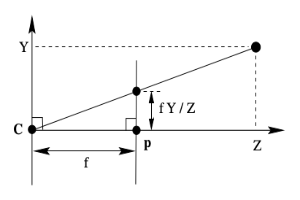
\includegraphics{proj1.png}
x= 0.5* film width* d/ focal length
    
y= 0.5* film height*d/ focal length

p1 = cam_pos + x* xcam + y* ycam + d* zcam

p2 = cam_pos + x* xcam - y* ycam + d* zcam

p3 = cam_pos - x* xcam - y* ycam + d* zcam

p4 = cam_pos - x* xcam + y* ycam + d* zcam 
    p1, p2, p3, p4 are the coordinates of the four corners for the
projective plane where x and y are the offset from the camera position.
To calculate the x and y, similar triangular rule was applied where d is
the distance between the camera to the target, in this case, point C to
Z. Focal length is shown as f in the image above. The distance beween
point Y and C is what we are trying to compute as x and y.

    \begin{Verbatim}[commandchars=\\\{\}]
{\color{incolor}In [{\color{incolor}19}]:} \PY{k}{def} \PY{n+nf}{plot\PYZus{}camera}\PY{p}{(}\PY{n}{ax}\PY{p}{,}\PY{n}{camera}\PY{p}{)}\PY{p}{:}
         	\PY{n}{cam1\PYZus{}pos}\PY{p}{,}\PY{n}{cam2\PYZus{}pos}\PY{p}{,}\PY{n}{target}\PY{p}{,}\PY{n}{up}\PY{p}{,}\PY{n}{focal\PYZus{}length}\PY{p}{,}\PY{n}{film\PYZus{}height}\PY{p}{,}
             \PY{n}{film\PYZus{}width}\PY{p}{,}\PY{n}{width}\PY{p}{,}\PY{n}{height}\PY{o}{=} \PY{n}{camera\PYZus{}specification}\PY{p}{(}\PY{p}{)}
         	\PY{k}{if} \PY{n}{camera}\PY{o}{==}\PY{l+m+mi}{1}\PY{p}{:}
         		\PY{n}{cam\PYZus{}pos}\PY{o}{=}\PY{n}{cam1\PYZus{}pos}
         		\PY{n}{color}\PY{o}{=}\PY{l+s+s1}{\PYZsq{}}\PY{l+s+s1}{r}\PY{l+s+s1}{\PYZsq{}}
         	\PY{k}{elif} \PY{n}{camera}\PY{o}{==}\PY{l+m+mi}{2}\PY{p}{:}
         		\PY{n}{cam\PYZus{}pos}\PY{o}{=}\PY{n}{cam2\PYZus{}pos}
         		\PY{n}{color}\PY{o}{=}\PY{l+s+s1}{\PYZsq{}}\PY{l+s+s1}{b}\PY{l+s+s1}{\PYZsq{}}
         	\PY{k}{else}\PY{p}{:}
         		\PY{k}{print} \PY{l+s+s1}{\PYZsq{}}\PY{l+s+s1}{the camera is not defined.}\PY{l+s+s1}{\PYZsq{}}
         	
         	\PY{n}{ax}\PY{o}{.}\PY{n}{scatter}\PY{p}{(}\PY{n}{cam\PYZus{}pos}\PY{p}{[}\PY{l+m+mi}{0}\PY{p}{]}\PY{p}{,}\PY{n}{cam\PYZus{}pos}\PY{p}{[}\PY{l+m+mi}{1}\PY{p}{]}\PY{p}{,}\PY{n}{cam\PYZus{}pos}\PY{p}{[}\PY{l+m+mi}{2}\PY{p}{]}\PY{p}{,}\PY{n}{marker}\PY{o}{=}\PY{l+s+s1}{\PYZsq{}}\PY{l+s+s1}{.}\PY{l+s+s1}{\PYZsq{}}\PY{p}{,}\PY{n}{c}\PY{o}{=}\PY{n}{color}\PY{p}{)}
         	
         	\PY{n}{xcam}\PY{p}{,}\PY{n}{ycam}\PY{p}{,}\PY{n}{zcam}\PY{o}{=} \PY{n}{camera\PYZus{}view\PYZus{}unit}\PY{p}{(}\PY{n}{target}\PY{p}{,}\PY{n}{cam\PYZus{}pos}\PY{p}{,}\PY{n}{up}\PY{p}{)}
             
         	\PY{c+c1}{\PYZsh{} four corners on the plane through focal points}
         	\PY{n}{d}\PY{o}{=} \PY{n}{np}\PY{o}{.}\PY{n}{linalg}\PY{o}{.}\PY{n}{norm}\PY{p}{(}\PY{n}{target}\PY{o}{\PYZhy{}}\PY{n}{cam\PYZus{}pos}\PY{p}{)}
         
         	\PY{n}{x}\PY{o}{=} \PY{l+m+mf}{0.5}\PY{o}{*} \PY{n}{film\PYZus{}width}\PY{o}{*}\PY{n}{d}\PY{o}{/}\PY{n}{focal\PYZus{}length}
         	\PY{n}{y}\PY{o}{=} \PY{l+m+mf}{0.5}\PY{o}{*} \PY{n}{film\PYZus{}height}\PY{o}{*}\PY{n}{d}\PY{o}{/}\PY{n}{focal\PYZus{}length}
         
         	\PY{n}{p1} \PY{o}{=} \PY{n}{cam\PYZus{}pos} \PY{o}{+} \PY{n}{x}\PY{o}{*} \PY{n}{xcam} \PY{o}{+} \PY{n}{y}\PY{o}{*} \PY{n}{ycam} \PY{o}{+} \PY{n}{d}\PY{o}{*} \PY{n}{zcam}
         	\PY{n}{p2} \PY{o}{=} \PY{n}{cam\PYZus{}pos} \PY{o}{+} \PY{n}{x}\PY{o}{*} \PY{n}{xcam} \PY{o}{\PYZhy{}} \PY{n}{y}\PY{o}{*} \PY{n}{ycam} \PY{o}{+} \PY{n}{d}\PY{o}{*} \PY{n}{zcam}
         	\PY{n}{p3} \PY{o}{=} \PY{n}{cam\PYZus{}pos} \PY{o}{\PYZhy{}} \PY{n}{x}\PY{o}{*} \PY{n}{xcam} \PY{o}{\PYZhy{}} \PY{n}{y}\PY{o}{*} \PY{n}{ycam} \PY{o}{+} \PY{n}{d}\PY{o}{*} \PY{n}{zcam}
         	\PY{n}{p4} \PY{o}{=} \PY{n}{cam\PYZus{}pos} \PY{o}{\PYZhy{}} \PY{n}{x}\PY{o}{*} \PY{n}{xcam} \PY{o}{+} \PY{n}{y}\PY{o}{*} \PY{n}{ycam} \PY{o}{+} \PY{n}{d}\PY{o}{*} \PY{n}{zcam}
         
         	\PY{c+c1}{\PYZsh{} connect these 4 points}
         	\PY{n}{plotx}\PY{o}{=}\PY{p}{[}\PY{n}{p1}\PY{p}{[}\PY{l+m+mi}{0}\PY{p}{]}\PY{p}{,}\PY{n}{p2}\PY{p}{[}\PY{l+m+mi}{0}\PY{p}{]}\PY{p}{,}\PY{n}{p3}\PY{p}{[}\PY{l+m+mi}{0}\PY{p}{]}\PY{p}{,}\PY{n}{p4}\PY{p}{[}\PY{l+m+mi}{0}\PY{p}{]}\PY{p}{,}\PY{n}{p1}\PY{p}{[}\PY{l+m+mi}{0}\PY{p}{]}\PY{p}{]}
         	\PY{n}{ploty}\PY{o}{=}\PY{p}{[}\PY{n}{p1}\PY{p}{[}\PY{l+m+mi}{1}\PY{p}{]}\PY{p}{,}\PY{n}{p2}\PY{p}{[}\PY{l+m+mi}{1}\PY{p}{]}\PY{p}{,}\PY{n}{p3}\PY{p}{[}\PY{l+m+mi}{1}\PY{p}{]}\PY{p}{,}\PY{n}{p4}\PY{p}{[}\PY{l+m+mi}{1}\PY{p}{]}\PY{p}{,}\PY{n}{p1}\PY{p}{[}\PY{l+m+mi}{1}\PY{p}{]}\PY{p}{]}
         	\PY{n}{plotz}\PY{o}{=}\PY{p}{[}\PY{n}{p1}\PY{p}{[}\PY{l+m+mi}{2}\PY{p}{]}\PY{p}{,}\PY{n}{p2}\PY{p}{[}\PY{l+m+mi}{2}\PY{p}{]}\PY{p}{,}\PY{n}{p3}\PY{p}{[}\PY{l+m+mi}{2}\PY{p}{]}\PY{p}{,}\PY{n}{p4}\PY{p}{[}\PY{l+m+mi}{2}\PY{p}{]}\PY{p}{,}\PY{n}{p1}\PY{p}{[}\PY{l+m+mi}{2}\PY{p}{]}\PY{p}{]}
         	
             \PY{c+c1}{\PYZsh{} plot the projective plane}
         	\PY{n}{verts}\PY{o}{=}\PY{p}{[}\PY{n+nb}{zip}\PY{p}{(}\PY{n}{plotx}\PY{p}{,}\PY{n}{ploty}\PY{p}{,}\PY{n}{plotz}\PY{p}{)}\PY{p}{]}
         	\PY{n}{face}\PY{o}{=}\PY{n}{Poly3DCollection}\PY{p}{(}\PY{n}{verts}\PY{p}{,}\PY{n}{alpha}\PY{o}{=}\PY{l+m+mf}{0.2}\PY{p}{,}\PY{n}{facecolors}\PY{o}{=}\PY{n}{color}\PY{p}{,}
                                   \PY{n}{linewidth}\PY{o}{=}\PY{l+m+mf}{0.5}\PY{p}{)}
         	
         	\PY{n}{ax}\PY{o}{.}\PY{n}{add\PYZus{}collection3d}\PY{p}{(}\PY{n}{face}\PY{p}{)}
         	\PY{n}{alpha}\PY{o}{=}\PY{l+m+mf}{0.2}
         	\PY{k}{if} \PY{n}{camera}\PY{o}{==}\PY{l+m+mi}{1}\PY{p}{:}
         		\PY{n}{face}\PY{o}{.}\PY{n}{set\PYZus{}facecolor}\PY{p}{(}\PY{p}{(}\PY{l+m+mi}{1}\PY{p}{,}\PY{l+m+mi}{0}\PY{p}{,}\PY{l+m+mi}{0}\PY{p}{,}\PY{n}{alpha}\PY{p}{)}\PY{p}{)}
         	\PY{k}{else}\PY{p}{:}
         		\PY{n}{face}\PY{o}{.}\PY{n}{set\PYZus{}facecolor}\PY{p}{(}\PY{p}{(}\PY{l+m+mi}{0}\PY{p}{,}\PY{l+m+mi}{0}\PY{p}{,}\PY{l+m+mi}{1}\PY{p}{,}\PY{n}{alpha}\PY{p}{)}\PY{p}{)}
         
             \PY{c+c1}{\PYZsh{} connect plane corner points to the camera}
         	\PY{n}{ax}\PY{o}{.}\PY{n}{plot}\PY{p}{(}\PY{p}{[}\PY{n}{cam\PYZus{}pos}\PY{p}{[}\PY{l+m+mi}{0}\PY{p}{]}\PY{p}{,}\PY{n}{target}\PY{p}{[}\PY{l+m+mi}{0}\PY{p}{]}\PY{p}{]}\PY{p}{,}\PY{p}{[}\PY{n}{cam\PYZus{}pos}\PY{p}{[}\PY{l+m+mi}{1}\PY{p}{]}\PY{p}{,}\PY{n}{target}\PY{p}{[}\PY{l+m+mi}{1}\PY{p}{]}\PY{p}{]}\PY{p}{,}
                     \PY{p}{[}\PY{n}{cam\PYZus{}pos}\PY{p}{[}\PY{l+m+mi}{2}\PY{p}{]}\PY{p}{,}\PY{n}{target}\PY{p}{[}\PY{l+m+mi}{2}\PY{p}{]}\PY{p}{]}\PY{p}{,}\PY{n}{c}\PY{o}{=}\PY{n}{color}\PY{p}{,}\PY{n}{linewidth}\PY{o}{=}\PY{l+m+mf}{0.3}\PY{p}{)}
         
         	\PY{n}{ax}\PY{o}{.}\PY{n}{plot}\PY{p}{(}\PY{p}{[}\PY{n}{cam\PYZus{}pos}\PY{p}{[}\PY{l+m+mi}{0}\PY{p}{]}\PY{p}{,}\PY{n}{p1}\PY{p}{[}\PY{l+m+mi}{0}\PY{p}{]}\PY{p}{]}\PY{p}{,}\PY{p}{[}\PY{n}{cam\PYZus{}pos}\PY{p}{[}\PY{l+m+mi}{1}\PY{p}{]}\PY{p}{,}\PY{n}{p1}\PY{p}{[}\PY{l+m+mi}{1}\PY{p}{]}\PY{p}{]}\PY{p}{,}
                     \PY{p}{[}\PY{n}{cam\PYZus{}pos}\PY{p}{[}\PY{l+m+mi}{2}\PY{p}{]}\PY{p}{,}\PY{n}{p1}\PY{p}{[}\PY{l+m+mi}{2}\PY{p}{]}\PY{p}{]}\PY{p}{,}\PY{n}{c}\PY{o}{=}\PY{n}{color}\PY{p}{,}\PY{n}{linewidth}\PY{o}{=}\PY{l+m+mf}{0.3}\PY{p}{)}
         	\PY{n}{ax}\PY{o}{.}\PY{n}{plot}\PY{p}{(}\PY{p}{[}\PY{n}{cam\PYZus{}pos}\PY{p}{[}\PY{l+m+mi}{0}\PY{p}{]}\PY{p}{,}\PY{n}{p2}\PY{p}{[}\PY{l+m+mi}{0}\PY{p}{]}\PY{p}{]}\PY{p}{,}\PY{p}{[}\PY{n}{cam\PYZus{}pos}\PY{p}{[}\PY{l+m+mi}{1}\PY{p}{]}\PY{p}{,}\PY{n}{p2}\PY{p}{[}\PY{l+m+mi}{1}\PY{p}{]}\PY{p}{]}\PY{p}{,}
                     \PY{p}{[}\PY{n}{cam\PYZus{}pos}\PY{p}{[}\PY{l+m+mi}{2}\PY{p}{]}\PY{p}{,}\PY{n}{p2}\PY{p}{[}\PY{l+m+mi}{2}\PY{p}{]}\PY{p}{]}\PY{p}{,}\PY{n}{c}\PY{o}{=}\PY{n}{color}\PY{p}{,}\PY{n}{linewidth}\PY{o}{=}\PY{l+m+mf}{0.3}\PY{p}{)}
         	\PY{n}{ax}\PY{o}{.}\PY{n}{plot}\PY{p}{(}\PY{p}{[}\PY{n}{cam\PYZus{}pos}\PY{p}{[}\PY{l+m+mi}{0}\PY{p}{]}\PY{p}{,}\PY{n}{p3}\PY{p}{[}\PY{l+m+mi}{0}\PY{p}{]}\PY{p}{]}\PY{p}{,}\PY{p}{[}\PY{n}{cam\PYZus{}pos}\PY{p}{[}\PY{l+m+mi}{1}\PY{p}{]}\PY{p}{,}\PY{n}{p3}\PY{p}{[}\PY{l+m+mi}{1}\PY{p}{]}\PY{p}{]}\PY{p}{,}
                     \PY{p}{[}\PY{n}{cam\PYZus{}pos}\PY{p}{[}\PY{l+m+mi}{2}\PY{p}{]}\PY{p}{,}\PY{n}{p3}\PY{p}{[}\PY{l+m+mi}{2}\PY{p}{]}\PY{p}{]}\PY{p}{,}\PY{n}{c}\PY{o}{=}\PY{n}{color}\PY{p}{,}\PY{n}{linewidth}\PY{o}{=}\PY{l+m+mf}{0.3}\PY{p}{)}
         	\PY{n}{ax}\PY{o}{.}\PY{n}{plot}\PY{p}{(}\PY{p}{[}\PY{n}{cam\PYZus{}pos}\PY{p}{[}\PY{l+m+mi}{0}\PY{p}{]}\PY{p}{,}\PY{n}{p4}\PY{p}{[}\PY{l+m+mi}{0}\PY{p}{]}\PY{p}{]}\PY{p}{,}\PY{p}{[}\PY{n}{cam\PYZus{}pos}\PY{p}{[}\PY{l+m+mi}{1}\PY{p}{]}\PY{p}{,}\PY{n}{p4}\PY{p}{[}\PY{l+m+mi}{1}\PY{p}{]}\PY{p}{]}\PY{p}{,}
                     \PY{p}{[}\PY{n}{cam\PYZus{}pos}\PY{p}{[}\PY{l+m+mi}{2}\PY{p}{]}\PY{p}{,}\PY{n}{p4}\PY{p}{[}\PY{l+m+mi}{2}\PY{p}{]}\PY{p}{]}\PY{p}{,}\PY{n}{c}\PY{o}{=}\PY{n}{color}\PY{p}{,}\PY{n}{linewidth}\PY{o}{=}\PY{l+m+mf}{0.3}\PY{p}{)}
\end{Verbatim}


    Plot the virtual world and the two set cameras with projective plane.
Camera 1 is in red while camera 2 is in blue color.

    \begin{Verbatim}[commandchars=\\\{\}]
{\color{incolor}In [{\color{incolor}15}]:} \PY{n}{ax}\PY{o}{=}\PY{n}{define\PYZus{}3Dpoints}\PY{p}{(}\PY{p}{)}
         \PY{n}{plt}\PY{o}{.}\PY{n}{show}\PY{p}{(}\PY{p}{)}
         \PY{n}{ax}\PY{o}{=}\PY{n}{define\PYZus{}3Dpoints}\PY{p}{(}\PY{p}{)}
         \PY{n}{plot\PYZus{}camera}\PY{p}{(}\PY{n}{ax}\PY{p}{,}\PY{l+m+mi}{1}\PY{p}{)}
         \PY{n}{plot\PYZus{}camera}\PY{p}{(}\PY{n}{ax}\PY{p}{,}\PY{l+m+mi}{2}\PY{p}{)}
         \PY{n}{plt}\PY{o}{.}\PY{n}{show}\PY{p}{(}\PY{p}{)}
\end{Verbatim}


    \begin{center}
    \adjustimage{max size={0.9\linewidth}{0.9\paperheight}}{output_17_0.png}
    \end{center}
    { \hspace*{\fill} \\}
    
    \begin{center}
    \adjustimage{max size={0.9\linewidth}{0.9\paperheight}}{output_17_1.png}
    \end{center}
    { \hspace*{\fill} \\}
    
    View the projection in different angles.

    \begin{Verbatim}[commandchars=\\\{\}]
{\color{incolor}In [{\color{incolor}11}]:} \PY{n}{ax}\PY{o}{=}\PY{n}{define\PYZus{}3Dpoints}\PY{p}{(}\PY{p}{)}
         \PY{n}{plot\PYZus{}camera}\PY{p}{(}\PY{n}{ax}\PY{p}{,}\PY{l+m+mi}{1}\PY{p}{)}
         \PY{n}{plot\PYZus{}camera}\PY{p}{(}\PY{n}{ax}\PY{p}{,}\PY{l+m+mi}{2}\PY{p}{)}
         \PY{n}{ax}\PY{o}{.}\PY{n}{view\PYZus{}init}\PY{p}{(}\PY{n}{elev}\PY{o}{=}\PY{l+m+mi}{35}\PY{p}{,}\PY{n}{azim}\PY{o}{=}\PY{l+m+mi}{65}\PY{p}{)}
         \PY{n}{plt}\PY{o}{.}\PY{n}{show}\PY{p}{(}\PY{p}{)}
\end{Verbatim}


    \begin{center}
    \adjustimage{max size={0.9\linewidth}{0.9\paperheight}}{output_19_0.png}
    \end{center}
    { \hspace*{\fill} \\}
    
    \begin{Verbatim}[commandchars=\\\{\}]
{\color{incolor}In [{\color{incolor}12}]:} \PY{n}{ax}\PY{o}{=}\PY{n}{define\PYZus{}3Dpoints}\PY{p}{(}\PY{p}{)}
         \PY{n}{plot\PYZus{}camera}\PY{p}{(}\PY{n}{ax}\PY{p}{,}\PY{l+m+mi}{1}\PY{p}{)}
         \PY{n}{plot\PYZus{}camera}\PY{p}{(}\PY{n}{ax}\PY{p}{,}\PY{l+m+mi}{2}\PY{p}{)}
         \PY{n}{ax}\PY{o}{.}\PY{n}{view\PYZus{}init}\PY{p}{(}\PY{n}{elev}\PY{o}{=}\PY{l+m+mf}{37.5}\PY{p}{,}\PY{n}{azim}\PY{o}{=}\PY{l+m+mi}{34}\PY{p}{)}
         \PY{n}{plt}\PY{o}{.}\PY{n}{show}\PY{p}{(}\PY{p}{)}
\end{Verbatim}


    \begin{center}
    \adjustimage{max size={0.9\linewidth}{0.9\paperheight}}{output_20_0.png}
    \end{center}
    { \hspace*{\fill} \\}
    
    \hypertarget{conclusion-and-discussion}{%
\section{Conclusion and Discussion}\label{conclusion-and-discussion}}

    To conclude, this exercise is to build a 3D virtual world with a set of
points. Then two cameras in different locations were added into the
world. The projective plane of each camera was calculated based on the
parameters of the camera. Specically, the plane was set by four corner
points computed by camera coordinate frame and similar triangle rule.

The exploration of this exercise is that instead of using MATLAB, I did
the work all in python. Since there are several convenient build-in
function which are relevant to camera setting in MATLAB, I cannot use it
directly in python. Therefore, I had to figure out some ways to display
the work in python reasonably.

    \hypertarget{reference}{%
\section{Reference}\label{reference}}

    Richard Hartley, Andrew Zisserman, ``Multiple View Geometry in Computer
View'', second edition, 2004


    % Add a bibliography block to the postdoc
    
    
    
    \end{document}
